\documentclass[11pt]{article}
\usepackage{hyperref}
\usepackage{amsthm}
\usepackage{amsmath}
\usepackage{amsfonts}
\usepackage{tikz}
\usepackage{ wasysym }

\newtheorem{example}{Example}


\author{}
\title{}

\begin{document}
%\maketitle
{\Large
%Change Document name to: Graded Homework 1\_Jacob\_Nicholas
\noindent NAME:  Nicholas Jacob\\ 
STUDENT ID: \# 113578513\\
GRADED HOMEWORK NUMBER: 3\\
COURSE: CS/DSA 4513 DATABASE MANAGEMENT\\ 
SECTION: ONLINE\\SEMESTER: FALL 2023\\
INSTRUCTOR:  DR. LE GRUENWALD\\
 SCORE:}

\newpage
\begin{enumerate} 
\item 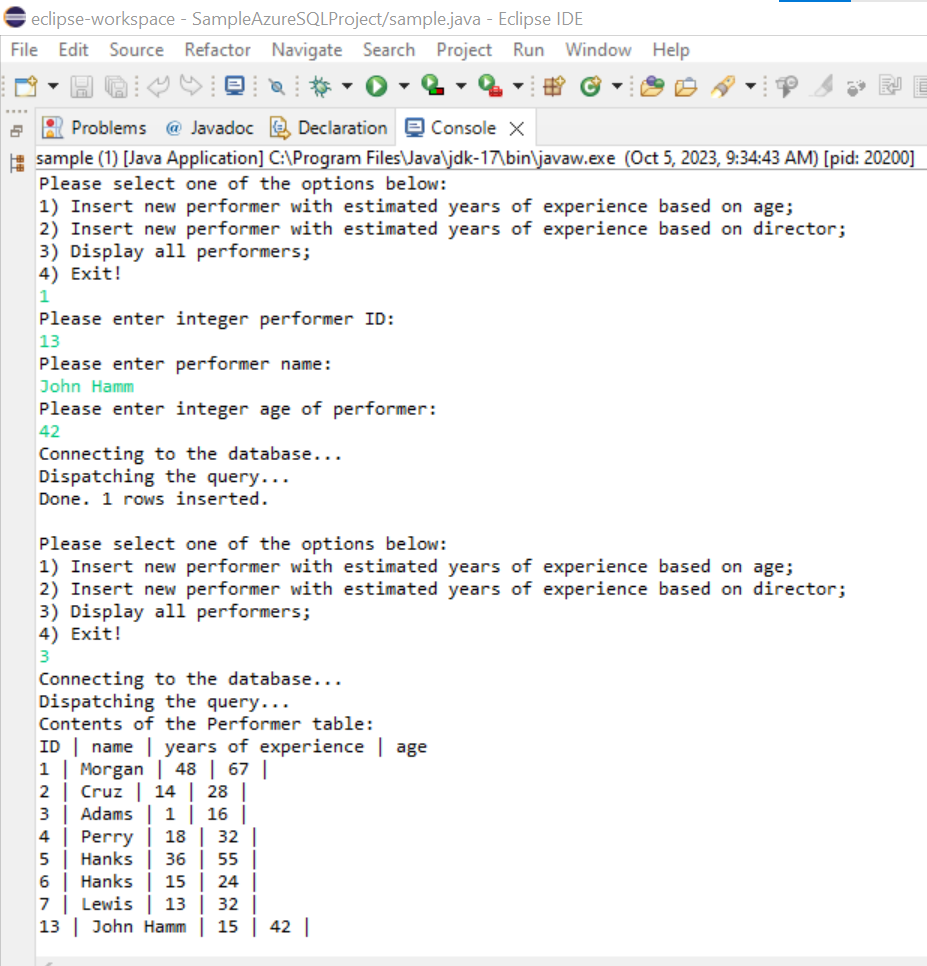
\includegraphics[width = \textwidth]{Insert1.png} 
\item 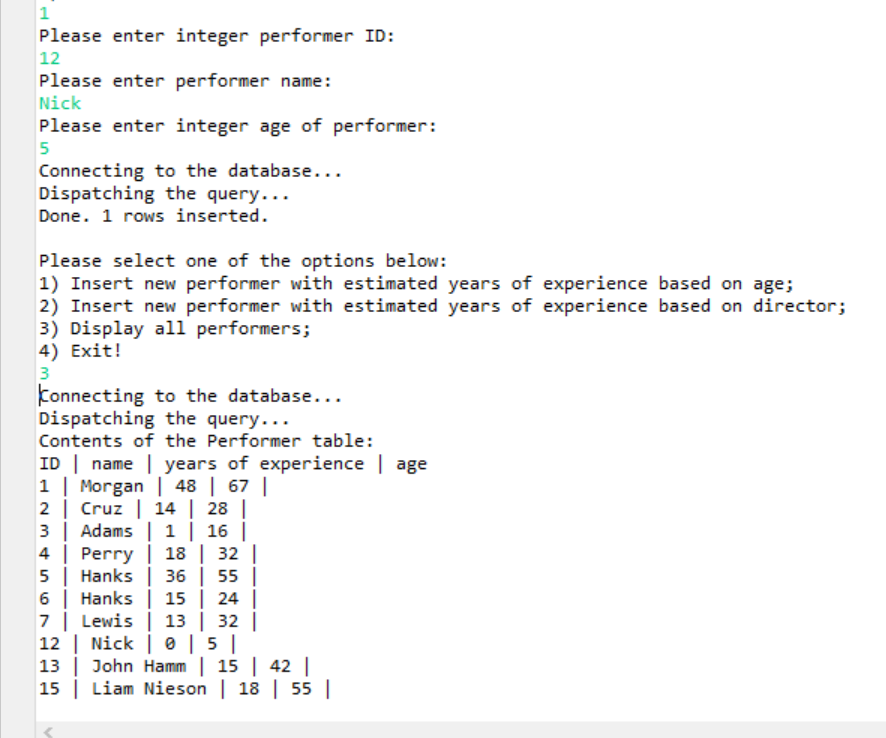
\includegraphics[width = \textwidth]{Insert1.1.png}
\item 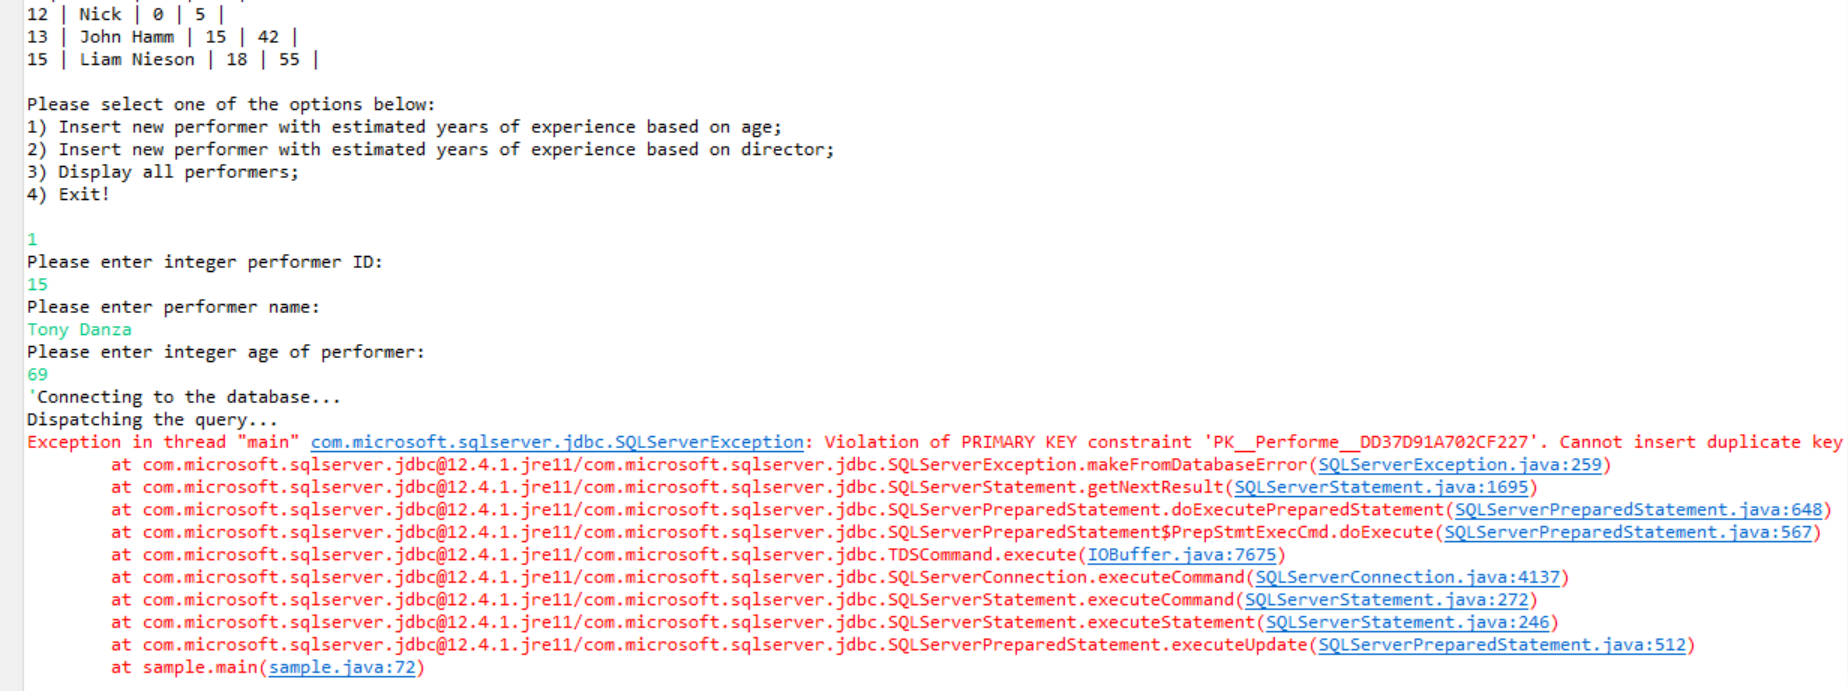
\includegraphics[width = \textwidth]{Insert1.2.DuplicateKeyError.png}  

\item 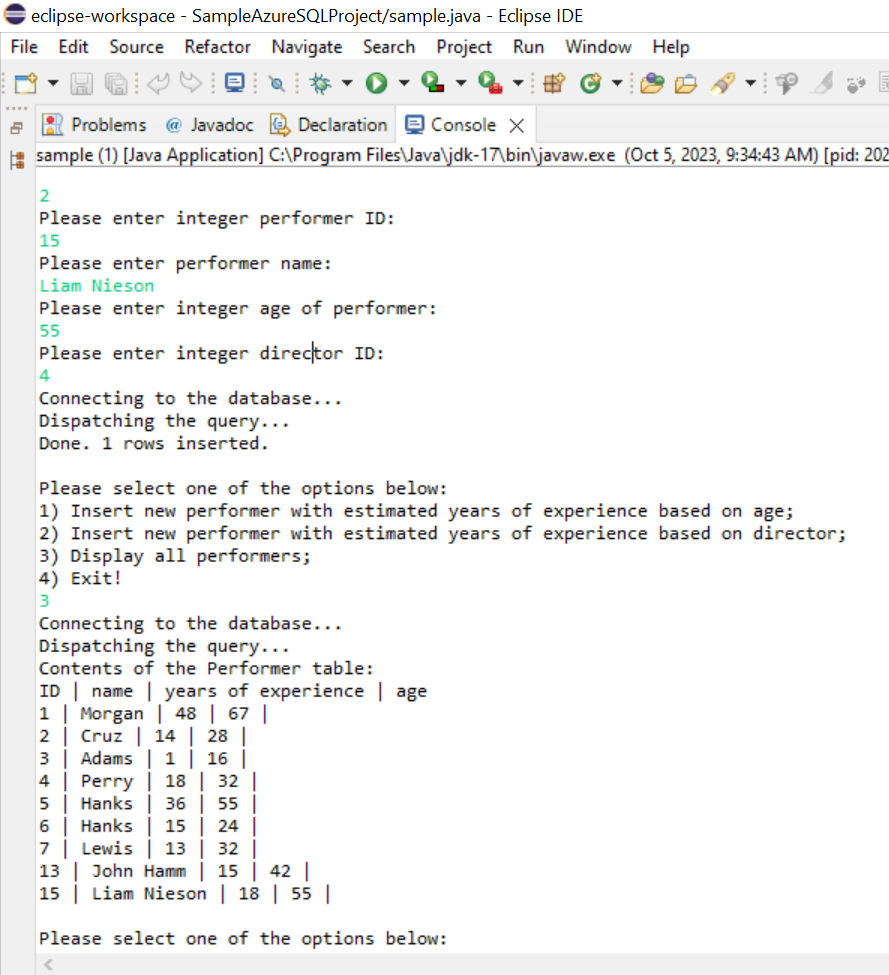
\includegraphics[width = \textwidth]{Insert2.png}
\item 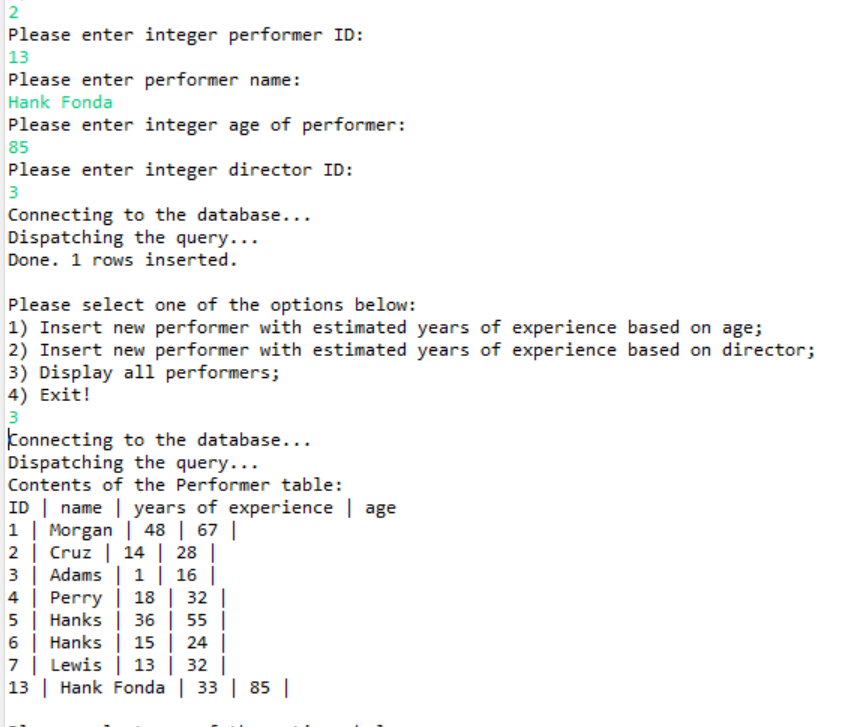
\includegraphics[width = \textwidth]{Insert2.1.png} 
\item 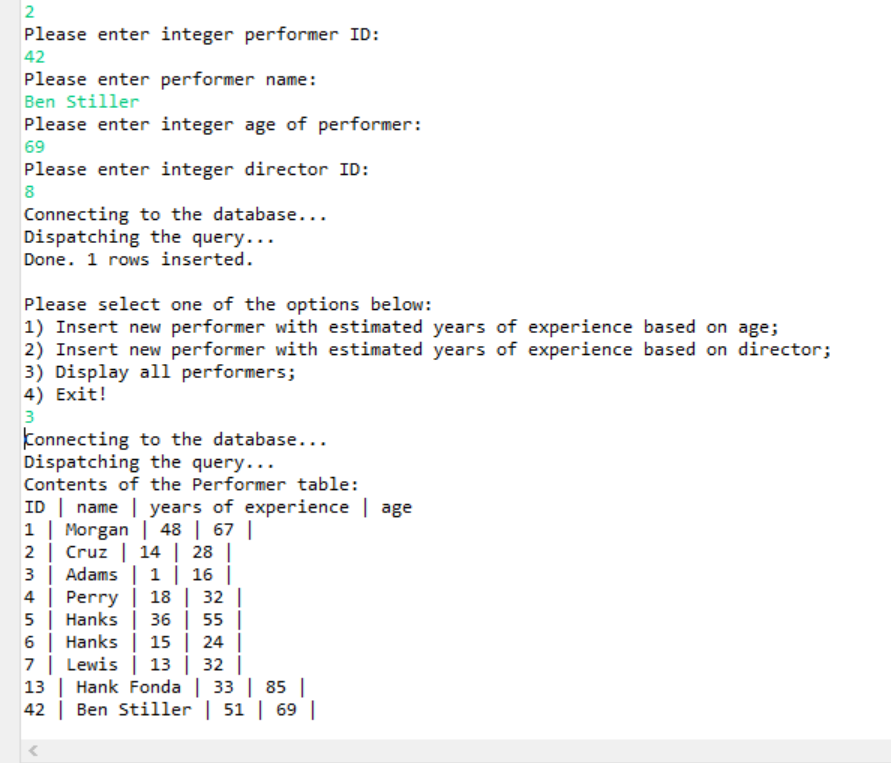
\includegraphics[width = \textwidth]{Insert2.2.png}
\item 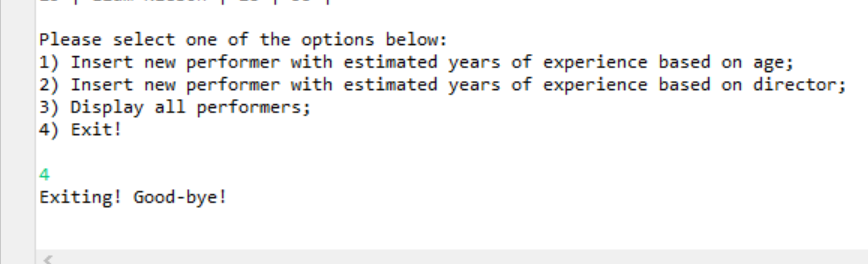
\includegraphics[width = \textwidth]{exiting.png}   


\end{enumerate}






\end{document}